%%%%%%%%%%%%%%%%%%%%%%%%%%%%%%%%%%%%%%%%%%%%%%%%%%%%%%%%%%%%%%%%%%%%%%%%%%%%%%%
% Projeto para concurso público de Pesquisador Adjunto I em Sismologia.
%
% Formatação inspirada em:
% * https://github.com/leouieda/memorial2023
% * https://github.com/birocoles/memos

%%%%%%%%%%%%%%%%%%%%%%%%%%%%%%%%%%%%%%%%%%%%%%%%%%%%%%%%%%%%%%%%%%%%%%%%%%%%%%%

%%%%%%%%%%%%%%%%%%%%%%%%%%%%%%%%%%%%%%%%%%%%%%%%%%%%%%%%%%%%%%%%%%%%%%%%%%%%%%%
% Set a class and import packages
\documentclass[10pt,a4paper,oneside]{book}

% Variables
\newcommand{\Year}{2024}
\newcommand{\Author}{Diogo Luiz de Oliveira Coelho}
\newcommand{\Title}{Projeto de \Author{} para concurso público - Pesquisador Adjunto I em Sismologia - ON/MCTI}
\newcommand{\Email}{diogoloc@on.br}
\newcommand{\EmailPersonal}{locdiogo@gmail.com}
\newcommand{\ORCID}{0000-0001-5426-0455}
\newcommand{\ResearchGate}{https://www.researchgate.net/profile/Diogo-De-Oliveira-Coelho}
\newcommand{\Lattes}{4330106475199471}

% Import packages
\usepackage[utf8]{inputenc}
\usepackage[T1]{fontenc}
\usepackage[brazil]{babel}
\usepackage{geometry}
\usepackage{graphicx}
\usepackage{amssymb}
\usepackage{amsmath}
\usepackage{mathpazo}
\usepackage{hyperref}
% create fancy headers
\usepackage{fancyhdr}
% commands for managing dates and its formats
\usepackage{datetime2}
% improved urls with proper hyphenation
\usepackage{xurl}
% Control over enumerate and itemize
\usepackage{enumitem}
% Tweak the look of captions
\usepackage{caption}
% To control the style of section titles
\usepackage{titlesec}
% Add the bibliography to the table of contents
\usepackage[nottoc,chapter]{tocbibind}
\usepackage[round,authoryear,sort]{natbib}
% show dois as links on references
\usepackage{doi}
% Icon and fonts (requires using xelatex or luatex)
\usepackage{fontawesome5}
\usepackage{academicons}
\usepackage{fontspec}
\usepackage[mono]{notomath}
% To make everything neater
\usepackage{microtype}
% To make fancy text boxes
\usepackage{xcolor}
\usepackage[framemethod=default]{mdframed}
% For fancy and multipage tables
\usepackage{tabularx}
\usepackage{ltablex}
% To define custom environments
\usepackage{environ}
\usepackage{setspace}
% Reference sections by name
\usepackage{nameref}
% Better handling of footnotes inside summary boxes
\usepackage{footmisc}

%to rotate the page
\usepackage{pdflscape}

%To plot piechart
\usepackage{bera}
\usepackage{pstricks-add}
\usepackage{pgf-pie}

\usepackage{wrapfig}

%%%%%%%%%%%%%%%%%%%%%%%%%%%%%%%%%%%%%%%%%%%%%%%%%%%%%%%%%%%%%%%%%%%%%%%%%%%%%%%

%%%%%%%%%%%%%%%%%%%%%%%%%%%%%%%%%%%%%%%%%%%%%%%%%%%%%%%%%%%%%%%%%%%%%%%%%%%%%%%
% Configuration of the document

\geometry{%
  left=30mm,
  right=30mm,
  top=20mm,
  bottom=15mm,
  headsep=5mm,
  headheight=5mm,
  footskip=10mm,
  includehead=true,
  includefoot=true
}

% Increase the line spacing
\SetSinglespace{1.2}
\onehalfspacing

% Remove spacing between enumerate/itemize items
\setlist{nosep}

% Padding between the first figure and the chapter title
\newcommand{\HeroFigPad}{\vspace{-1cm}}

% Padding before the software logo figures
\newcommand{\SoftwareFigPad}{\vspace{-0.3cm}}

% Add a link to a DOI
\newcommand{\DOI}[1]{\url{https://doi.org/#1}}

% Add a link to a GitHub repository
\newcommand{\GitHub}[1]{\faGithub{} Código: \url{https://github.com/#1}}

% Add a link to a YouTube video
\newcommand{\YouTube}[1]{\faYoutube{} Vídeo: \url{https://youtu.be/#1}}

% Add a link to a supplementary data
\newcommand{\Data}[1]{\faChartBar{} Dados: \url{https://doi.org/#1}}

% Add a link to a preprint
\newcommand{\Preprint}[1]{\faLockOpen{} Preprint: \url{https://doi.org/#1}}

% Make a Unicode bullet symbol
\newcommand{\Bullet}{•\enspace}

% Define custom colors
\definecolor{lu_gray}{gray}{0.98}
\definecolor{lu_darkgray}{gray}{0.3}
\definecolor{gold(metallic)}{rgb}{0.83, 0.69, 0.22}
\definecolor{cornsilk}{rgb}{1.0, 0.97, 0.86}
\definecolor{lu_blue}{RGB}{32, 96, 194}
\definecolor{lu_lightblue}{RGB}{238, 245, 250}
\definecolor{timberwolf}{rgb}{0.86, 0.84, 0.82}
\definecolor{battleshipgrey}{rgb}{0.52, 0.52, 0.51}

% Customize how Chapter headings are displayed
\titleformat{\chapter}[display]{\normalfont}{\large Capítulo \thechapter}{0pt}{\huge}[\titlerule]
\titlespacing*{\chapter}{0pt}{-40pt}{40pt}

% Set the spacing between bibliography entries (requires natbib)
\setlength{\bibsep}{0pt}

% Configure captions
\captionsetup{labelfont=bf,font={small,color=lu_darkgray},skip=0pt}

% Define a fancy text for summarybox
\mdfdefinestyle{summarybox}{%
  leftline=true,
  rightline=false,
  topline=false,
  bottomline=false,
  linewidth=4pt,
  linecolor=gold(metallic),
  frametitlefont=\bfseries\color{black}\small,
  frametitlebackgroundcolor=cornsilk,
  frametitleaboveskip=7pt,
  frametitlebelowskip=7pt,
  frametitlerule=true,
  frametitlerulewidth=1pt,
  backgroundcolor=lu_gray,
  innertopmargin=7pt,
  innerbottommargin=10pt,
  innerleftmargin=15pt,
  innerrightmargin=15pt,
  skipbelow=5pt,
  skipabove=0pt,
}
\newmdenv[style=summarybox]{summarybox}

% Define a fancy text for subsummarybox
\mdfdefinestyle{subsummarybox}{%
  leftline=true,
  rightline=false,
  topline=false,
  bottomline=false,
  linewidth=4pt,
  linecolor=battleshipgrey,
  frametitlefont=\bfseries\color{black}\small,
  frametitlebackgroundcolor=timberwolf,
  frametitleaboveskip=7pt,
  frametitlebelowskip=7pt,
  frametitlerule=true,
  frametitlerulewidth=1pt,
  backgroundcolor=lu_gray,
  innertopmargin=7pt,
  innerbottommargin=10pt,
  innerleftmargin=15pt,
  innerrightmargin=15pt,
  skipbelow=5pt,
  skipabove=0pt,
}
\newmdenv[style=subsummarybox]{subsummarybox}

% Define a fancy text for projectbox
\mdfdefinestyle{projectbox}{%
  leftline=true,
  rightline=false,
  topline=false,
  bottomline=false,
  linewidth=4pt,
  linecolor=lu_blue,
  frametitlefont=\bfseries\color{black}\small,
  frametitlebackgroundcolor=lu_lightblue,
  frametitleaboveskip=7pt,
  frametitlebelowskip=7pt,
  frametitlerule=true,
  frametitlerulewidth=1pt,
  backgroundcolor=lu_gray,
  innertopmargin=7pt,
  innerbottommargin=10pt,
  innerleftmargin=15pt,
  innerrightmargin=15pt,
  skipbelow=5pt,
  skipabove=0pt,
}
\newmdenv[style=projectbox]{projectbox}

% Define something like an fa-ul and a date list
\NewEnviron{fa-ul}{%
  \vspace{-0.4cm}
  \small
  \renewcommand{\arraystretch}{1.25}
  \begin{tabularx}{\linewidth}{@{}p{0.05\linewidth}@{}@{}p{0.95\linewidth}@{}}
    \BODY
  \end{tabularx}%
}
\NewEnviron{datelist}{%
  \vspace{-0.4cm}
  \small
  \renewcommand{\arraystretch}{1.25}
  \begin{tabularx}{\linewidth}{@{}p{0.15\linewidth}@{}@{}p{0.85\linewidth}@{}}
    \BODY
  \end{tabularx}%
}
\NewEnviron{paperlist}{%
  \vspace{-0.4cm}
  \small
  \renewcommand{\arraystretch}{1.25}
  \begin{tabularx}{\linewidth}{@{}p{0.08\linewidth}@{}@{}p{0.92\linewidth}@{}}
    \BODY
  \end{tabularx}%
}
\NewEnviron{courselist}{%
  \vspace{-0.4cm}
  \small
  \renewcommand{\arraystretch}{1.25}
  \begin{tabularx}{\linewidth}{@{}p{0.15\linewidth}@{}@{}p{0.85\linewidth}@{}}
    \BODY
  \end{tabularx}
}

% Define a fancy enumerate that has a title
\NewEnviron{fancyenum}[2]{%
  \vspace{0.25cm}
  \noindent#1\quad\textbf{#2}:
  \vspace{0.25cm}
  \begin{enumerate}
    \BODY
  \end{enumerate}
}

% Configure hyperref and add PDF metadata
\hypersetup{
    colorlinks,
    allcolors=lu_blue,
    pdftitle={\Title},
    pdfauthor={\Author},
    pdftex,
    breaklinks=true,
}

% make urls use the same font as every other text
\urlstyle{same}

% Prevent footnotes from being broken into multiple pages
\interfootnotelinepenalty=10000

% Configure headers and footers
\fancyhf{}
\lhead{\fontsize{9pt}{0}\selectfont\itshape \nouppercase\leftmark}
\chead{}
\rhead{\fontsize{9pt}{0}\selectfont \thepage}
\cfoot{}
\renewcommand{\headrulewidth}{0.3pt}
%%%%%%%%%%%%%%%%%%%%%%%%%%%%%%%%%%%%%%%%%%%%%%%%%%%%%%%%%%%%%%%%%%%%%%%%%%%%%%%

%%%%%%%%%%%%%%%%%%%%%%%%%%%%%%%%%%%%%%%%%%%%%%%%%%%%%%%%%%%%%%%%%%%%%%%%%%%%%%%
\begin{document}

\pagestyle{plain}
\frontmatter

\begin{titlepage}
  \begin{center}
    \includegraphics[height=2cm]{images/logo_terra.png}
    \vspace{1cm}

    CONCURSO PÚBLICO
    
    PESQUISADOR ADJUNTO I EM SISMOLOGIA
    
    OBSERVATÓRIO NACIONAL

    \vspace{5cm}

    \textbf{\LARGE Proposta de projeto de pesquisa}
    \vspace{1cm}

    \textbf{\LARGE \MakeUppercase{\Author{}}}
    \vspace{5cm}

    {\small
	Apresentado para concurso público de provas e títulos para cargo de

	Pesquisador Adjunto I em Sismologia do Observatório Nacional.
      \vspace{1cm}

	EDITAL N$^{\circ}$   1, DE 9 DE OUTUBRO DE 2023
    }
    \vfill

    \Year{}
  \end{center}
\end{titlepage}

%==============================================================================
\chapter*{Resumo}

Ao longo da minha trajetória acadêmica, obtive sucesso ao concluir o bacharelado em \href{https://geologia.ufes.br/}{Geologia} pela Universidade Federal do Espírito Santo, o mestrado em \href{https://www.gov.br/observatorio/pt-br/assuntos/programas-academicos/pos-graduacao-em-geofisica/pos-graduacao-em-geofisica}{Geofísica} pelo Observatório Nacional e o doutorado em \href{https://posgraduacao.ufrn.br/325}{Geodinâmica e Geofísica} pela Universidade Federal do Rio Grande do Norte. Durante minha formação acadêmica, tive a oportunidade de passar por três instituições de ensino superior ligadas ao Ministério da Educação (MEC), uma unidade de pesquisa vinculada ao Ministério da Ciência, Tecnologia e Inovações (MCTI), além de realizar estágio de nível superior na Petrobras, uma empresa estatal do setor de energia. Nessa caminhada acadêmica, tive a oportunidade enriquecedora de vivenciar de perto instituições públicas em quatro estados distintos do país. Essa diversidade geográfica proporcionou-me um aprendizado valioso e o aprimoramento da minha atuação na academia. Desde minha entrada no Observatório Nacional, ministrei a disciplina de \href{https://www.gov.br/observatorio/pt-br/assuntos/programas-academicos/pos-graduacao-em-geofisica/grade-curricular}{Introdução à Sismologia} em nível de pós-graduação, cursos de curta duração para graduandos em outras instituições e orientei alunos de iniciação científica. No âmbito da divulgação e popularização da ciência, redigi diversas notas técnicas tanto para a instituição quanto para veículos de imprensa. Além disso, participei de mais de 35 eventos relacionados a popularização e divulgação da ciência, dentre feiras de tecnologia, entrevistas para diversos canais da imprensa, podcast, revisão de textos e notas técnicas explorando temas variados da sismologia, incluindo sua relação com desastres naturais, bem como curiosidades gerais da população sobre a atuação de um pesquisador em geofísica. Desde o mestrado, tenho atuado na área de Sismologia e Tectônica da Crosta. Já no doutorado iniciei, de forma sistemática, o processo de desenvolvimento de diversos códigos em \href{https://www.python.org/}{python} para a sismologia, incluindo \href{https://github.com/dIOGOLOC/codes_escritos/tree/master/mantle_transition_zone_migration_obspy_Pds}{Receiver Migration}, \href{https://zooxantelapy.readthedocs.io/en/latest/}{Zooxantelapy} e \href{https://github.com/dIOGOLOC/marefone/wiki}{Marefone}. O primeiro pacote está relacionado a estruturação do manto terrestre e os dois últimos à dados oriundos de redes subaquáticas, às quais iniciei o tratamento e processamento de dados em 2020. Este memorial apresenta de forma resumida minha formação e atuação acadêmica, incluindo algumas considerações sobre os fatores que influenciaram na minha trajetória e os principais ensinamentos adquiridos ao longo dessa jornada que me ajudaram fazer pequenos ajustes na rota até aqui.

\begin{landscape}
% Conteúdo da página em modo paisagem
\begin{figure}[tb]
\begin{center}
\includegraphics[width=\pagewidth]{images/linha_do_projeto.png}
\end{center}
\caption*{Resumo cronológico dos temas a serem desenvolvidos. Borda completa: plena capacidade de desenvolvimento e experiência prática, Borda incompleta: necessidade de aperfeiçoamento de metodologias e experiência prática incompleta, Borda tracejada: falta de arcabouço teórico e prático.}
\label{fig_tempo_linha}
\end{figure}
\end{landscape}
%==============================================================================
\tableofcontents

\mainmatter
\pagestyle{fancy}

%==============================================================================
\chapter{Apresentação}

\begin{minipage}[b]{0.5\linewidth}
{\faUser} \textbf{Identificação:} Diogo Luiz de Oliveira Coelho\\
{\faIcon{at}} \textbf{e-mail profissional:}  \href{mailto:\Email}{\Email} \\
{\faIcon{at}} \textbf{e-mail pessoal:}  \href{mailto:\EmailPersonal}{\EmailPersonal}\\
\textbf{Links úteis: }  
\href{https://orcid.org/\ORCID}{\Large \aiOrcid}
\href{\ResearchGate}{\Large \aiResearchGate}
\href{https://lattes.cnpq.br/\Lattes}{\Large \aiLattes}
\href{https://github.com/diogoloc}{\Large \faIcon{github}}
\end{minipage}
\begin{minipage}[b]{0.5\linewidth}
\centering
\includegraphics[scale=0.1]{images/foto.jpg}
\end{minipage}

\bigskip	
\bigskip	
\bigskip	
\bigskip	

\begin{summarybox}[frametitle=\faAward{}\quad Resumo da formação e atuação acadêmica]
  \begin{datelist}
    2007--2012 & Bacharelado em Geologia (UFES) \\
    2013--2015 & Mestrado em Geofísica (ON) \\
    2015--2019 & Doutorado em Geodinâmica e Geofísica (UFRN) \\
    2020--2021 & Estágio Pós-doutoral I (UFSC) \\
    2022--2023 & Estágio Pós-doutoral II  (ON) \\
    2023--atual & Estágio Pós-doutoral III (ON)
  \end{datelist}
\end{summarybox}

\bigskip	

A presente proposta de projeto de pesquisa representa um esforço dedicado à investigação e avanço de áreas da sismologia brasileira, principalmente quando se refere à parte acústica e hidroacústica. Este projeto tem como objetivo preencher lacunas identificadas previamente, visando a ampliação e aprofundamento da compreensão nessas áreas desafiadoras, que possuem grande potencial para trabalhos interdisciplinares. Com base na revisão da literatura e na identificação de questões ainda não exploradas, esta proposta visa desenvolver uma série de estudos inovadores que possam agregar valor teórico e prático à comunidade científica, além de aumentar a área de contato com temas relevantes para a sociedade civil. Com uma abordagem interdisciplinar, o projeto visa não apenas responder a perguntas específicas de pesquisa, mas também promover o diálogo interdisciplinar e a colaboração entre diferentes áreas de conhecimento relacionadas aos diversos temas abordados.

%==============================================================================

\chapter{Estrutura do Projeto}
\label{cap_estrutura}

\begin{figure}[h]
	\HeroFigPad
	\begin{center}
		\includegraphics[width=\textwidth]{images/arpoador.jpg}
	\end{center}
	\caption{
	O pôr do sol no \href{https://pt.wikipedia.org/wiki/Arpoador}{Arpoador} serviu de inspiração para a concepção deste Projeto de Pesquisa, uma vez que representa um espetáculo fenomenal que une o céu, o mar e a terra.
    }
 \label{fig_arpoador}
\end{figure}

Como o Projeto de pesquisa possui várias frentes de atuação em ambientes distintos, para facilitar a leitura e o acopanhamento dos projetos de pesquisa propostos, estruturei o plano em três capítulos diferentes, cada um associado com um elemento da Figura \ref{fig_arpoador}, Mar (capítulo \ref{cap_mar}), Terra (capítulo \ref{cap_terra}) e Céu (capítulo \ref{cap_ceu}), além de posicionar cronologicamente os ambientes e projetos.

\bigskip

\begin{summarybox}[frametitle=\faStreetView{}\quad Panorama cronológico dos temas propostos]
  \begin{datelist}
    2024--2028 & Monitoramento sísmico e hidroacústico (MAR) \\
    2024--2028 & Ilhas oceânicas (MAR) \\
    2025--2030 & Estrutura profunda do Brasil (TERRA) \\
    2028--2030 & Monitoramento de barragens (TERRA) \\
    2034--2040 & Monitoramento infrassônico (CÉU) 
  \end{datelist}
\end{summarybox}

\bigskip

Observando o resumo cronológico inicial da minha proposta, é possível identificar uma sequência de temas prospostos com diferentes prazos de implementação. Esses períodos evidenciam lacunas acadêmicas, metodológicas ou práticas, por parte do autor. Por exemplo, considerando o caso do monitoramento com o uso de equipamentos de infrassom, até o momento não possuo experiência prática com esse tipo de dado. Por essa razão, na linha do tempo, ele é o último tema a ser iniciado. No entanto, como descreverei no plano de implementação (capítulo \ref{cap_ceu}), essa falta de experiência pode ser sanada através de um cronograma estruturado de ações para aumentar a minha experiência neste tema. Notadamente observa-se um alinhamento cronológico com a \href{http://www.finep.gov.br/images/contratos-Adm/2022/dou/Y_S_dias_extrato_contrato.pdf}{expansão para o mar da Rede Sismográfica Brasileira} e os projetos aqui propostos. Pois, além de participar do grupo de execução dessa expansão, eu tenho experiências com esse tipo de banco de dados e tenho plena convicção da necessidade de implementação de novas frentes de trabalho para enfrentar os desafios desse tipo de projeto.

Nem todos os temas de projetos exemplificados nesta proposta estão em fase embrionária. Por exemplo, o tema que visa estudar as Ilhas oceânicas, já está sendo executado e já tem resultados promissores, com mostra o trabalho apresentado no 18$^\circ$ Congresso Internacional da Sociedade Brasileira de Geofísica\footnote{Resumo (2023): 18th International Congress of the Brazilian Geophysical Society, Rio de Janeiro, Brazil. \href{https://sbgf.org.br/mysbgf/eventos/expanded_abstracts/18th_CISBGf/57aeee35c98205091e18d1140e9f38cfShort_Abstract_18th_CISBGf_.docx}{Comparison of the shallow and deep structure beneath the Abrolhos Archipelago and the Trindade Island with passive-source seismology}. Eveline Sayao, Diogo Luiz de Oliveira Coelho, Daniele Ingredy Gomes Silva, Carlos Ribeiro, Sergio Luiz Fontes, Thiago Santanna, Elisabeth Lima, Ronaldo Marins}. Outro tema que já está estruturado é o Estruturua profunda do Brasil, onde já formamos um grupo de pesquisa com pesquisadores e alunos de algumas universidade para atualizar metodologias e propor ideias de trabalhos para estudar a estrutura profunda de certas áreas do Brasil com dados da \href{http://rsbr.on.br/}{RSBR}. 

Para facilitar o acompanhamento das várias propostas de projetos de pesquisa, cada um dos projetos foram estruturados segundo a tabela abaixo, onde todos os projetos possuem um título, justificativa, objetivos, metodologia, bibliografia e plano de implementação. 

\bigskip

\begin{subsummarybox}[frametitle=\faBullhorn\quad Constituição de cada projeto]
  \begin{fa-ul}
    \faTag & \textbf{Título:} Tema do projeto \\
    \faBook & \textbf{Bibliografia básica:} Referências de trabalhos fundamentais \\
    \faPencil* &  \textbf{Justificativa:} Relevância da pesquisa \\
	\faDatabase & \textbf{Banco de Dados:} Referência do banco de dados utilizado \\
    \faFutbol & \textbf{Objetivos:} Tópicos o que se pretende pesquisar \\
    \faBrain & \textbf{Plano de Implementação:} Etapas de como realizar a pesquisa  \\
    \faShoppingCart & \textbf{Produtos:} Lista com os principais resultados do projeto
  \end{fa-ul}
\end{subsummarybox}

%==============================================================================

\chapter{Mar}
\label{cap_mar}

\begin{figure}[h]
	\HeroFigPad
	\begin{center}
		\includegraphics[width=\textwidth]{images/obs_foto.jpeg}
	\end{center}
	\caption{
	Processo de instalação de um Sismômetro de Fundo Ocêanico no \href{https://sismo-oceano.ufsc.br/}{Projeto Monitoramento Sismo-Oceanográfico}.
    }
 \label{fig_obs}
\end{figure}

Neste capítulo, apresento de forma resumida os projetos que serão realizados para investigar a estrutura profunda do Brasil através de uma gama de metodologias consolidas, dentre as quais temos: \href{https://doi.org/10.1029/JB084iB09p04749}{Função do Receptor}, \href{https://doi.org/10.1111/j.1365-246X.1990.tb04573.x}{Dispersão de Ondas de Superfície}, \href{https://doi.org/10.1046/j.1365-246x.2000.00217.x}{Inversão Conjunta}, \href{https://doi.org/10.1016/j.epsl.2013.08.025}{Migração das Funções do Receptor} e \href{https://doi.org/10.1111/j.1365-246X.2007.03374.x}{Tomografia de Ruído Sísmico}.   

\section{Tema: Monitoramento Sísmico e Hidroacústico}

Como demonstrado no memorial, eu tenho experiência no processamento de banco de dados sísmicos e acústicos orindos de equipamentos oceânicos, como: sismômetros de fundo oceânico (\href{https://en.wikipedia.org/wiki/Ocean-bottom_seismometer}{OBS}), sismógrafos flutuantes (\href{https://www.geoazur.fr/GLOBALSEIS/Mermaid.html}{MERMAID}) e planadores oceânicos (\href{https://oceanservice.noaa.gov/facts/ocean-gliders.html}{GLIDER}). Após a análise desses banco de dados, sugere-se um projeto que tenha foco em metodologias de redução/supressão de ruído nos dados.

\subsection{Projeto: Redução de ruído em dados sísmicos e acústicos}

A proposta de redução de ruído se faz necessária devido ao alto nível de ruído basal encontrado globalmente em dados de equipamentos localizados em áreas oceânicas (Bayrakci \& Klingelhoefer, 2024). Devido alta sensibilidade de Sismômetros de Fundo Oceânico (OBS), o nível de ruído nesses dados é bem elevado devido a várias condicionantes (e.g. correntes de fundo oceânico, baixo acoplamento entre o sensor e o assoalho oceânico, operações submarinas próximas, etc). Existem metodologias recentes, como o trabalho de Zali et al. (2023), para a redução de ruído nos dados de OBS através de algoritmos de processamento de áudio, onde os resultados encontrados são bem satisfatórios. Para dados acústicos, temos o trabalho de Shen et al. (2024) que mostra observações de ondas T de terremotos distantes e regionais e um esquema de supressão de ruído por Curvelet para aprimorar os sinais de ondas T. No entanto, nossa ideia não é utilizar somente a transformada Curvelet, e sim utilizar a combinação das transformadas de Wavelet e Curvelet para lidar com as fraquezas individuais de cada método e suprimir ruído dos dados, como mostra Bal et al.(2019) a remoção de ruído nas imagens de Tomografia por Emissão de Pósitrons (PET).

\begin{fancyenum}{\faDatabase}{Banco de Dados}
	\item Sismômetros de Fundo Oceânico: \href{https://sismo-oceano.ufsc.br/}{Bacia de Campos e Santos} (\faLock);
	\item Planadores Submarinos: \href{https://comunicabaciadesantos.petrobras.com.br/projeto-de-monitoramento-da-paisagem-acustica-submarina-pmpas-}{Bacia de Santos} (\faLock);
	\item Hidrofones acoplados em linhas de fundeio: \href{https://comunicabaciadesantos.petrobras.com.br/projeto-de-monitoramento-da-paisagem-acustica-submarina-pmpas-}{Bacia de Santos} (\faLock);
	\item Sismógrafos flutuantes: \href{https://www.geoazur.fr/GLOBALSEIS/Data.html}{Ilha de Galápagos} (\faUnlock).
	\item Hidrofones do \href{https://www.ctbto.org/our-work/international-monitoring-system}{Sistema de Monitoramento Internacional}: \href{https://ds.iris.edu/gmap/\#network=IM\&planet=earth}{Incorporated Research Institution for Seismology} (\faUnlock);

\end{fancyenum}

\begin{fancyenum}{\faFutbol}{Objetivos}
	\item Aplicar métodos de processamento de áudio para remoção de ruído em dados sísmicos;
	\item Aplicar métodos de processamento de imagem para remoção de ruído em dados acústicos;
	\item Combinar as transformadas de Wavelet e Curvelet para aprimorar os sinais das \href{https://insu.hal.science/insu-00915042/document}{ondas T} nos dados acústicos.
\end{fancyenum}

\begin{fancyenum}{\faBrain}{Plano de Implementação}
	\item Compilação dos dados acústicos e sísmicos disponíveis;
	\item Compilação de pacotes eficientes em python para o desenvolvimento dos algoritmos computacionais;
	\item Testes com sintéticos utilizando \href{https://pyrocko.org/docs/current/apps/fomosto/tutorial.html}{FOMOSTO} e \href{https://ds.iris.edu/ds/products/syngine/}{SYNGINE}, ferramentas que fornecem acesso a sismogramas de acordo com funções de Green e modelos de Terra pré-calculados;
	\item Testes em dados reais;
	\item Elaboração de documentação do pacote computacional e dos algoritmos desenvolvidos.
\end{fancyenum}

\begin{fancyenum}{\faShoppingCart}{Produtos}
	\item Desenvolvimento de algoritmos computacionais para a remoção de ruídos em dados sísmicos e acústicos;
	\item Implementação de pacote computacional em python para compilar os algoritmos criados.
\end{fancyenum}

\begin{fancyenum}{\faBook}{Bibliografia básica}
	\item Bal, A., Banerjee, M., Sharma, P. et al. 2019. An efficient wavelet and curvelet-based PET image denoising technique. Med Biol Eng Comput 57, 2567–2598. https://doi.org/10.1007/s11517-019-02014-w;
	\item Bayrakci, G. and Klingelhoefer, F. 2024. eds. Noisy Oceans. Geophysical Monograph Series. Wiley, 28 February 2024. https://doi.org/10.1002/9781119750925;
	\item Shen, Z., \& Wu, W. 2024. Ocean bottom distributed acoustic sensing for oceanic seismicity detection and seismic ocean thermometry. Journal of Geophysical Research: Solid Earth, 129,e2023JB027799. https://doi.org/10.1029/
2023JB027799;
	\item Zali, Z., Rein, T., Krüger, F., Ohrnberger, M., and Scherbaum, F. 2023. Ocean bottom seismometer (OBS) noise reduction from horizontal and vertical components using harmonic–percussive separation algorithms, Solid Earth, 14, 181–195, https://doi.org/10.5194/se-14-181-2023.
\end{fancyenum}

\subsection{Projeto: Localização de eventos sísmicos utilizando reflexões hidroacústicas}

Eventos de grande amplitude, como explosões e terremotos, produzem sinais hidroacústicos de grande amplitude que têm sido estudados desde a Segunda Guerra Mundial. Upton et al. (2006) mostra que quando o som viaja na coluna d'água e encontra uma mudança na impedância, como um monte submarino, uma ilha ou uma plataforma continental, parte da energia pode ser dispersada ou refletida. Como relata Hanson \& Bowman (2006), é notável a eficiência da propagação hidroacústica nos oceanos. As reflexões hidroacústicas oriundas de grandes alvos batimétricos podem ser usadas para restringir as localizações de eventos quando a cobertura da estação não é ideal. Dados hidroacústicos históricos e contemporâneos de muitas explosões subaquáticas e terremotos sub-marinhos mostram grandes reflexões chegando aos receptores dezenas de minutos ou horas após a chegada direta (Upton et al., 2006). Devido a isso, o objetivo deste estudo é investigar a possibilidade de melhorar/localizar eventos hidroacústicos locais registrados por hidrofones instalados na costa sudeste do Brasil. 

\begin{fancyenum}{\faDatabase}{Banco de Dados}
	\item Hidrofones acoplados em OBS: \href{https://sismo-oceano.ufsc.br/}{Bacia de Campos e Santos} (\faLock);
	\item Hidrofones acoplados em linhas de fundeio: \href{https://comunicabaciadesantos.petrobras.com.br/projeto-de-monitoramento-da-paisagem-acustica-submarina-pmpas-}{Bacia de Santos} (\faLock);
	\item Planadores Submarinos: \href{https://comunicabaciadesantos.petrobras.com.br/projeto-de-monitoramento-da-paisagem-acustica-submarina-pmpas-}{Bacia de Santos} (\faLock).
	\item Hidrofones do \href{https://www.ctbto.org/our-work/international-monitoring-system}{Sistema de Monitoramento Internacional}: \href{https://ds.iris.edu/gmap/\#network=IM\&planet=earth}{Incorporated Research Institution for Seismology} (\faUnlock);
\end{fancyenum}

\begin{fancyenum}{\faFutbol}{Objetivos}
	\item Identificar as reflexões hidroacústicas de grandes eventos sísmicos locais;
	\item Identificar as principais feições batimétricas que podem ser potencias fontes de reflexões hidroacústicas;
	\item Avaliar a viabilidade do uso de reflexões hidroacústicas para localizar eventos sísmicos locais;
	\item Estender o potencial de cobertura de detecção e localização da Rede Sismográfica Brasileira.
\end{fancyenum}

\begin{fancyenum}{\faBrain}{Plano de Implementação}
	\item Idenficação de potenciais sinais refletidos em sismogramas;
	\item Associação destes eventos com as feiçõess batimétricas proeminentes que podem atuar como superfícies refletoras;
	\item O tempo de viagem entre o refletor e o sensor é previsto usando um modelo de velocidade do som oceânico dependente da estação;
	\item As chegadas diretas e refletidas são então usadas como entrada para o algoritmo de localização padrão, conforme descrito acima.
\end{fancyenum}

\begin{fancyenum}{\faShoppingCart}{Produtos}
	\item Melhoramento da determinação da localização de grandes terremotos locais, utilizando as fases sísmicas e acústicas;
	\item Pacote computacional eficiente em python para localizar os eventos.
\end{fancyenum}

\begin{fancyenum}{\faBook}{Bibliografia básica}
	\item Hanson, J. A. and Bowman, J.R.  2006. Methods for monitoring hydroacoustic events using direct and reflected T waves in the Indian Ocean, J. Geophys. Res., 111, B02305, doi:10.1029/2004JB003609.
	\item Upton, Z.M., Pulli, J.J., Myhre, B., Blau, D. 2006. A reflected energy prediction model for long-range hydroacoustic reflection in the oceans. J Acoust Soc Am. 2006 Jan;119(1):153-60. doi: 10.1121/1.2141234.
\end{fancyenum}

\subsection{Projeto: Instalação de estação hidroacústica de baixo custo - tríade de hidrofones}

O \href{https://www.ctbto.org/our-work/international-monitoring-system}{Sistema de Monitoramento Internacional} da \href{https://funag.gov.br/biblioteca/download/934-Tratado_de_Proibicao_Completa_dos_Testes_Nucleares_CTBT.pdf}{Organização do Tratado de Proibição Completa de Testes Nucleares} e Gibbons (2022) descrevem um bom exemplo de estação hidroacústica para o monitoramento de eventos sísmicos submarinos. O \href{https://www.ctbto.org/our-work/monitoring-technologies/hydroacoustic-monitoring}{array de hidrofones} consiste de uma ou duas redes triangulares de hidrofones submersos diretamente no canal \href{https://pt.wikipedia.org/wiki/Canal_SOFAR}{SOFAR}. Esse tipo de estação é chamado de estação de fase-T, referente a onda Terciária (T), em uma convenção de nomenclatura consistente com as ondas sísmicas primárias (P) e secundárias (S). A justificativa para o implantação desse tipo de estação é o custo, pois para implantar e manter esse tipo de estação é bem menor que o custo de um sismômetro de fundo oceânico. Essa tríade de hidrofones podem medir a velocidade de fase, direção e coerência das fases acústicas, e ajudam a determinar a localização da fonte sísmica. Devido à natureza coerente da propagação de ondas sonoras no oceano e à permanência de um canal bem definido de velocidade do som oceânico (SOFAR), as tríades de hidrofones proporcionam uma melhoria significativa no limiar de detecção e na precisão da localização de eventos sísmicos, podendo detectar eventos sísmicas a distâncias de até dezesseis mil quilômetros (Prior et al., 2011). Os sinais recebidos do mesmo evento nos três hidrofones são correlacionados para fornecer tempos de atraso entre as chegadas do evento para determinar o azimute no qual o sinal chegou (Gibbons, 2022).

\begin{fancyenum}{\faDatabase}{Banco de Dados}
	\item Dados para teste no \href{https://www.ctbto.org/our-work/international-monitoring-system}{Sistema de Monitoramento Internacional}: \href{https://ds.iris.edu/gmap/\#network=IM\&planet=earth}{Incorporated Research Institution for Seismology} (\faUnlock);
\end{fancyenum}

\begin{fancyenum}{\faFutbol}{Objetivos}
	\item Identificar os pontos ideais de instalação da estação hidroacústica para otimizar a composição da Rede Sismográfica Brasileira no Mar;
	\item Avaliar a viabilidade de equipamentos e infraestrutura de baixo custo na implantação da estação;
	\item Avaliar a viabilidade de utilizar o mesmo equipamento para estudos multidisciplinares relacionados à ciências do mar;
	\item Estender o potencial de cobertura de detecção e localização de eventos pela Rede Sismográfica Brasileira no mar.
\end{fancyenum}


\begin{fancyenum}{\faBrain}{Plano de Implementação}
	\item Coletar e analisar os dados de outras estações para buscar a melhor configuração de equipamentos e local de instalação;
	\item Identificar fontes de financiamento adequadas para o projeto, com a possibilidade de inserção em projeto interdisciplinares;
	\item Definir a área de cobertura desejada e os tipos de eventos a serem detectados;
	\item Identificar potenciais locais de instalação e levar em conta fatores como profundidade da lâmica d'água, fontes de ruído e segurança das instalações (e.g. rotas de navios) pois estes interferem no custo do projeto;
	\item Adquirir os hidrofones e equipamentos de baixo custo operacional.
\end{fancyenum}

\begin{fancyenum}{\faShoppingCart}{Produtos}
	\item Melhoramento da cobertura azimutal da Rede Sismográfica Brasileira no mar;
	\item Melhorar a detecção e localização de grandes terremotos locais na Costa Brasileira.
\end{fancyenum}

\begin{fancyenum}{\faBook}{Bibliografia básica}
	\item Prior, M. K., Meless, O., Bittner,P. and H. Sugioka, H. 2011. Long-Range Detection and Location of Shallow Underwater Explosions Using Deep-Sound-Channel Hydrophones. IEEE Journal of Oceanic Engineering, vol. 36, no. 4, pp. 703-715, doi: 10.1109/JOE.2011.2154390.
	\item Gibbons, S.J. 2022. The Hydroacoustic Network of the CTBT International Monitoring System: Access and Exploitation, Journal for Peace and Nuclear Disarmament, 5:2, 452-468, DOI: 10.1080/25751654.2022.2129948.
\end{fancyenum}


\section{Tema: Ilhas Oceânicas}

\subsection{Projeto: Estrutura rasa e profunda abaixo de Ilhas oceânicas (Abrolhos, Trindade e Tristão da Cunha)}

The Earth's surface is dynamic, the result of several moving lithospheric plates overlying a plastically flowing asthenosphere, where these plates can pull apart, collide, or slide one another along faults. Tectonic processes generate several geological features, like mountains, volcanoes, sedimentary basins, lakes, and faults, among others. However, an island or archipelago is a geologically anomalous feature found at ocean basins; and one of the biggest challenges to understand its origin is the mismatch between its orientation/shape and the regional fracture zones trends. Understanding the shallow and deep Earth architecture beneath these emergent land features is a key point for improving our comprehension about ongoing and past geological processes in these areas. Lithospheric-scale processes, such as the origin and evolution of islands, leave behind a trail of footprints on the subsurface that can be retrieved by geophysical methods. Our study area is located at the Brazilian continental margin, which includes several volcanic islands and submerged volcanic seamounts related to post-breakup magmatic episodes. The Abrolhos Archipelago is a group of small islands with a semi-circular shape composed of igneous bodies on the continental shelf at different depth. The Trindade Island corresponds to the easternmost island of the submarine E-W Vitória-Trindade Chain, composed of seamounts, guyots and oceanic islands starting 175 km off the coast of Espírito Santo State and extending for 950 km eastward. The main goal of our study is to compare the shallow and deep structure beneath these emergent land areas and highlight seismic discontinuities, in order to improve our understanding of its architecture and help constrain models for its origin and evolution. Due to the technical difficulties to maintain a permanent station far away from the continent, each island has only one seismic broadband station working, thus we implement robust methodologies for single station measurements, including stochastic methods and deep learning. The dataset has been collected from two permanent broadband stations of the Brazilian Seismographic Network (RSBR) installed at the islands. Regarding the shallow structure, we calculated the Fundamental Frequency (f0) using the horizontal-to-vertical spectral ratio (HVSR) technique, which is normally used to retrieve information about the subsoil seismic properties. In the case of deep structure constraints, the receiver function technique (RF) is one of the most successful methodologies in broadband seismology for imaging of the crust and mantle. We expect to infer details about the architecture of the crust and mantle beneath the islands and contribute towards a better understanding of the role of magmatic processes and the thermal and mechanical properties of the lithosphere

\begin{fancyenum}{\faDatabase}{Banco de Dados}
	\item Dados para teste no \href{https://www.ctbto.org/our-work/international-monitoring-system}{Sistema de Monitoramento Internacional}: \href{https://ds.iris.edu/gmap/\#network=IM\&planet=earth}{Incorporated Research Institution for Seismology} (\faUnlock);
\end{fancyenum}

\begin{fancyenum}{\faFutbol}{Objetivos}
	\item Identificar os pontos ideais de instalação da estação hidroacústica para otimizar a composição da Rede Sismográfica Brasileira no Mar;
	\item Avaliar a viabilidade de equipamentos e infraestrutura de baixo custo na implantação da estação;
	\item Avaliar a viabilidade de utilizar o mesmo equipamento para estudos multidisciplinares relacionados à ciências do mar;
	\item Estender o potencial de cobertura de detecção e localização de eventos pela Rede Sismográfica Brasileira no mar.
\end{fancyenum}


\begin{fancyenum}{\faBrain}{Plano de Implementação}
	\item Coletar e analisar os dados de outras estações para buscar a melhor configuração de equipamentos e local de instalação;
	\item Identificar fontes de financiamento adequadas para o projeto, com a possibilidade de inserção em projeto interdisciplinares;
	\item Definir a área de cobertura desejada e os tipos de eventos a serem detectados;
	\item Identificar potenciais locais de instalação e levar em conta fatores como profundidade da lâmica d'água, fontes de ruído e segurança das instalações (e.g. rotas de navios) pois estes interferem no custo do projeto;
	\item Adquirir os hidrofones e equipamentos de baixo custo operacional.
\end{fancyenum}

\begin{fancyenum}{\faShoppingCart}{Produtos}
	\item Melhoramento da cobertura azimutal da Rede Sismográfica Brasileira no mar;
	\item Melhorar a detecção e localização de grandes terremotos locais na Costa Brasileira.
\end{fancyenum}

\begin{fancyenum}{\faBook}{Bibliografia básica}
	\item Prior, M. K., Meless, O., Bittner,P. and H. Sugioka, H. 2011. Long-Range Detection and Location of Shallow Underwater Explosions Using Deep-Sound-Channel Hydrophones. IEEE Journal of Oceanic Engineering, vol. 36, no. 4, pp. 703-715, doi: 10.1109/JOE.2011.2154390.
	\item Gibbons, S.J. 2022. The Hydroacoustic Network of the CTBT International Monitoring System: Access and Exploitation, Journal for Peace and Nuclear Disarmament, 5:2, 452-468, DOI: 10.1080/25751654.2022.2129948.
\end{fancyenum}

% ==============================================================================
\chapter{Terra}
\label{cap_terra}

\begin{figure}[h]
	\HeroFigPad
	\begin{center}
		\includegraphics[width=\textwidth]{images/globe_structure.jpg}
	\end{center}
	\caption{
	Modelo tomográfico global do manto superior. \href{https://www.olcf.ornl.gov/2017/03/28/a-seismic-mapping-milestone/}{Fonte}.
    }
 \label{fig_structure}
\end{figure}

Neste capítulo, apresento de forma resumida os projetos que serão realizados para investigar a estrutura profunda do Brasil através de uma gama de metodologias consolidas, dentre as quais temos: \href{https://doi.org/10.1029/JB084iB09p04749}{Função do Receptor}, \href{https://doi.org/10.1111/j.1365-246X.1990.tb04573.x}{Dispersão de Ondas de Superfície}, \href{https://doi.org/10.1046/j.1365-246x.2000.00217.x}{Inversão Conjunta}, \href{https://doi.org/10.1016/j.epsl.2013.08.025}{Migração das Funções do Receptor} e \href{https://doi.org/10.1111/j.1365-246X.2007.03374.x}{Tomografia de Ruído Sísmico}.   

\section{Tema: Estrutura profunda do Brasil}

\begin{summarybox}[frametitle=\faProjectDiagram{}\quad Panorama da linha de pesquisa]
	\begin{datelist}
		\faFile* & \textbf{Número de projetos:} 4 \\
		\faBinoculars & \textbf{Equipamentos:} Sismômetros banda larga e período curto \\
		\faCalendar*[regular] & \textbf{Período:} 2013 - atual \\
		\faMapMarked* & \textbf{Regiões:} Faixa Ribeira, Bacia do Parnaíba, ilhas oceânicas e bacias costeiras. \\
	\end{datelist}
\end{summarybox}

\bigskip

Esta linha de pesquisa busca revelar a estruturação profunda da Terra através de uma gama de metodologias, dentre as quais temos: \href{https://doi.org/10.1029/JB084iB09p04749}{Função do Receptor}, \href{https://doi.org/10.1111/j.1365-246X.1990.tb04573.x}{Dispersão de Ondas de Superfície}, \href{https://doi.org/10.1046/j.1365-246x.2000.00217.x}{Inversão Conjunta}, \href{https://doi.org/10.1016/j.epsl.2013.08.025}{Migração das Funções do Receptor} e \href{https://doi.org/10.1111/j.1365-246X.2007.03374.x}{Tomografia de Ruído Sísmico}. Esta linha de pesquisa está intimamente ligada à minha trajetória acadêmica, uma vez que minha formação prévia em Geologia, combinada com os resultados obtidos pelos métodos sismológicos, contribuem para uma visão abrangente da composição e dinâmica da subsuperfície terrestre. A caracterização da estrutura profunda das bacias cratônicas, faixas móveis e cratons permitem a identificação de padrões de sedimentação, processos geodinâmicos associados e processos de formação de montanhas, falhas e outros elementos estruturais. Além disso, a investigação da estrutura do manto superior, principalmente da zona de transição, fornece informações cruciais sobre a composição, temperatura e movimentos do manto superior, contribuindo para o entendimento dos processos de convecção e circulação mantélica que impulsionam a dinâmica global do planeta.  

\begin{fancyenum}{\faFutbol}{Objetivos}
	\item Imagear as principais descontinuidades crustais e mantélicas;
	\item Caracterizar a estrutura crustal profunda das principais provincias geológicas do Brasil;
	\item Investigar a composição, temperatura e fluxos do manto superior;
	\item Desenvolver rotinas computacionais mais eficientes para estimar as profundidade e espessuras das camadas em subsuperfície.
\end{fancyenum}

\begin{fancyenum}{\faCogs}{Principais contribuições}
	\item Estimativas da espessura das principais camadas abaixo de bacias intracratônicas;
	\item Contribuições no entendimento dos processos profundos atuantes em bacias sedimentares intracratônicas no Brasil;
	\item Rotina computacional para o cálculo das Funções do Receptor de onda P inteiramente em python;
	\item Programa eficiente para realizar a migração pré-empilhamento das Funções do Receptor de onda P.
\end{fancyenum}
% ==============================================================================

\chapter{Céu}
\label{cap_ceu}

\begin{figure}[h]
	\HeroFigPad
	\begin{center}
		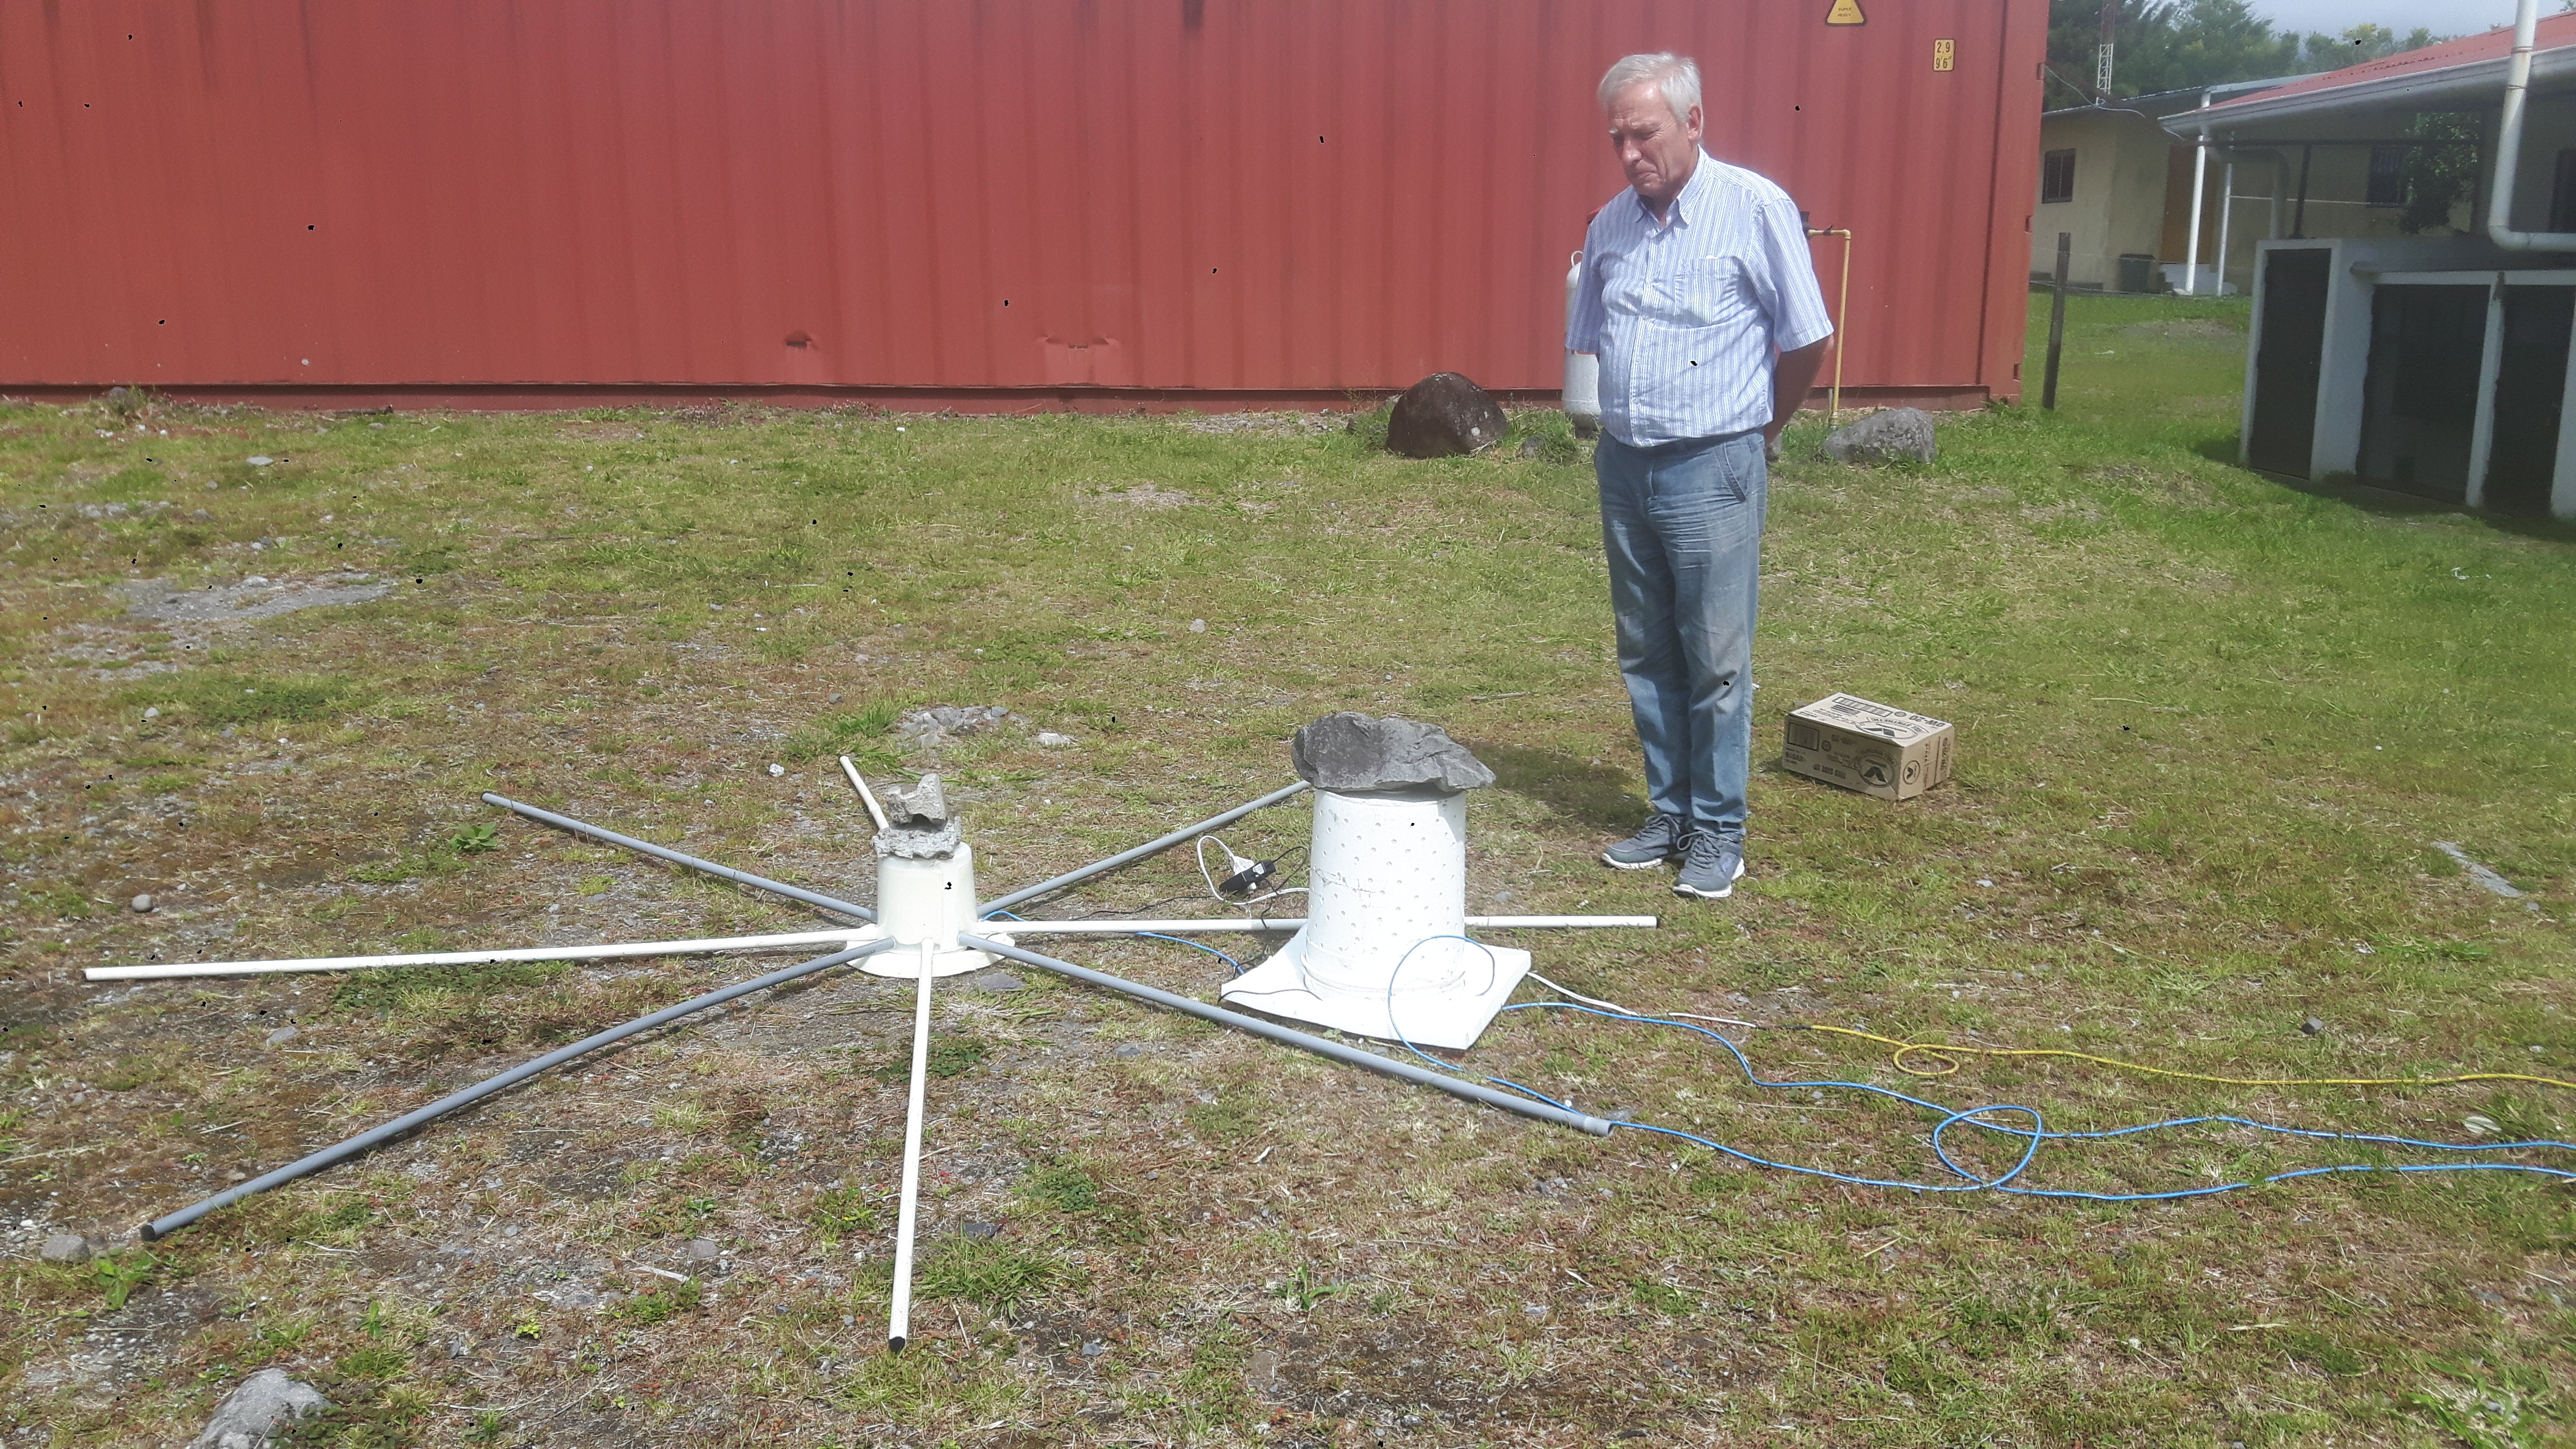
\includegraphics[width=\textwidth]{images/wind_infrasound.jpg}
	\end{center}
	\caption{
	Instação de um Raspberry Boom, uma inovação significativa no campo da monitoramento de infrassom. Tecnologia avançada e acessível ($\approx$ 1000 USD), que ofere uma maneira eficaz de detectar e analisar ondas sonoras de baixa frequência geradas por eventos naturais e antrópicos. Na foto observa-se um formato conhecido como \href{https://www.ctbto.org/our-work/monitoring-technologies/infrasound-monitoring}{pipe arrays}, empregado pela Organização do Tratado de Proibição Completa de Testes Nucleares (\href{https://www.ctbto.org/}{CTBTO}) para a supressão do ruído do vento nos dados.
    }
 \label{fig_wind}
\end{figure}

Observar ondas sonoras propagadas pelo ar é uma área crucial em diversos campos, desde a acústica e engenharia de som até a meteorologia e monitoramento ambiental. Essas ondas, resultantes de variações na pressão do ar, carregam uma riqueza de informações sobre fontes sonoras, características do ambiente e fenômenos naturais. Em resumo, a análise de ondas sonoras pelo ar é uma ferramenta poderosa e versátil que desempenha um papel vital em uma variedade de campos. Ao compreender como as ondas sonoras se comportam no ambiente atmosférico, podemos obter insights valiosos sobre uma ampla gama de fenômenos naturais e antrópicos, promovendo avanços significativos em diversas áreas das geociências.

\section{Tema: Monitoramento Infrassônico}

\subsection{Projeto: Instalação de estação de infrassom de baixo custo no Rio de Janeiro}

O \href{https://www.ctbto.org/our-work/international-monitoring-system}{Sistema de Monitoramento Internacional} da \href{https://funag.gov.br/biblioteca/download/934-Tratado_de_Proibicao_Completa_dos_Testes_Nucleares_CTBT.pdf}{Organização do Tratado de Proibição Completa de Testes Nucleares} e Gibbons (2022) descrevem um bom exemplo de estação hidroacústica para o monitoramento de eventos sísmicos submarinos. O \href{https://www.ctbto.org/our-work/monitoring-technologies/hydroacoustic-monitoring}{array de hidrofones} consiste de uma ou duas redes triangulares de hidrofones submersos diretamente no canal \href{https://pt.wikipedia.org/wiki/Canal_SOFAR}{SOFAR}. Esse tipo de estação é chamado de estação de fase-T, referente a onda Terciária (T), em uma convenção de nomenclatura consistente com as ondas sísmicas primárias (P) e secundárias (S). A justificativa para o implantação desse tipo de estação é o custo, pois para implantar e manter esse tipo de estação é bem menor que o custo de um sismômetro de fundo oceânico. Essa tríade de hidrofones podem medir a velocidade de fase, direção e coerência das fases acústicas, e ajudam a determinar a localização da fonte sísmica. Devido à natureza coerente da propagação de ondas sonoras no oceano e à permanência de um canal bem definido de velocidade do som oceânico (SOFAR), as tríades de hidrofones proporcionam uma melhoria significativa no limiar de detecção e na precisão da localização de eventos sísmicos, podendo detectar eventos sísmicas a distâncias de até dezesseis mil quilômetros (Prior et al., 2011). Os sinais recebidos do mesmo evento nos três hidrofones são correlacionados para fornecer tempos de atraso entre as chegadas do evento para determinar o azimute no qual o sinal chegou (Gibbons, 2022).

\begin{fancyenum}{\faDatabase}{Banco de Dados}
	\item Dados para teste no \href{https://www.ctbto.org/our-work/international-monitoring-system}{Sistema de Monitoramento Internacional}: \href{https://ds.iris.edu/gmap/\#network=IM\&planet=earth}{Incorporated Research Institution for Seismology} (\faUnlock);
\end{fancyenum}

\begin{fancyenum}{\faFutbol}{Objetivos}
	\item Identificar os pontos ideais de instalação da estação hidroacústica para otimizar a composição da Rede Sismográfica Brasileira no Mar;
	\item Avaliar a viabilidade de equipamentos e infraestrutura de baixo custo na implantação da estação;
	\item Avaliar a viabilidade de utilizar o mesmo equipamento para estudos multidisciplinares relacionados à ciências do mar;
	\item Estender o potencial de cobertura de detecção e localização de eventos pela Rede Sismográfica Brasileira no mar.
\end{fancyenum}


\begin{fancyenum}{\faBrain}{Plano de Implementação}
	\item M;
	\item Associação destes eventos com as feiçõess batimétricas proeminentes que podem atuar como superfícies refletoras;
	\item O tempo de viagem entre o refletor e o sensor é previsto usando um modelo de velocidade do som oceânico dependente da estação;
	\item As chegadas diretas e refletidas são então usadas como entrada para o algoritmo de localização padrão, conforme descrito acima.
\end{fancyenum}

\begin{fancyenum}{\faShoppingCart}{Produtos}
	\item Melhoramento da cobertura azimutal da Rede Sismográfica Brasileira no mar;
	\item Melhorar a detecção e localização de grandes terremotos locais na Costa Brasileira.
\end{fancyenum}

\begin{fancyenum}{\faBook}{Bibliografia básica}
	\item Prior, M. K., Meless, O., Bittner,P. and H. Sugioka, H. 2011. Long-Range Detection and Location of Shallow Underwater Explosions Using Deep-Sound-Channel Hydrophones. IEEE Journal of Oceanic Engineering, vol. 36, no. 4, pp. 703-715, doi: 10.1109/JOE.2011.2154390.
	\item Gibbons, S.J. 2022. The Hydroacoustic Network of the CTBT International Monitoring System: Access and Exploitation, Journal for Peace and Nuclear Disarmament, 5:2, 452-468, DOI: 10.1080/25751654.2022.2129948.
\end{fancyenum}

%==============================================================================

\chapter{Considerações Finais}
\label{cap_conclusao}

Este memorial narra minha jornada desde os meados dos anos 2000, quando iniciei meu curso de Geologia na Universidade Federal do Espírito Santo, até meu último estágio pós-doutoral no Observatório Nacional, instituição que desempenhou um papel fundamental ao longo da minha trajetória acadêmica. Durante meu último estágio pós-doutoral nessa instituição, pude aprofundar meu conhecimento e contribuir para projetos de pesquisa de grande relevância. Nessa maratona acadêmica, passei por 4 instituições federais em 4 estados diferentes, visitei 15 estados para participar de conferências nacionais e aulas de campo e visitei 5 países assistindo a cursos e conferências internacionais graças ás oportunidades geradas pelos programas de pós-graduação, projetos e bolsas que estive envolvidos.

\begin{figure}
	\centering
	\begin{tikzpicture}
	\pie{34.3/Entrevista escrita (13),
		21.0/Entrevista gravada (8),
		10.5/Revisão de texto (4),
		7.8/Evento Online (3), 
		7.8/Entrevista ao vivo (3),
		5.2/Evento presencial (2),
		5.2/Mini-curso (2),
		8/Outros (3)}
	\end{tikzpicture}
	\caption{Estatística das atividades de divulgação científicas realizadas entre 2020 e 2024.}
	\label{fig_resumo_divulgacao}
\end{figure}

Os números apresentados acima, assim como a lista \ref{lista_divulgacao}, fornecem uma visão detalhada dessa abordagem multifacetada na popularização da ciência e das atividades do Obseravtório Nacional ao longo do período que estive na instituição, um total de 38 atividades ao longo de 3 anos. Destaco que concedi dezenas de entrevistas, totalizando 24 (13 escritas, 8 gravadas e 3 ao vivo), contribuí revisando textos na temática da Sismologia e Geologia que foram publicados nas redes sociais do Obseravtório Nacional. Além disso, fiz parte da comitiva que participou do \href{https://www.gov.br/observatorio/pt-br/assuntos/areas-de-atuacao/divulgacao-e-popularizacao-da-ciencia/on-riw}{Rio Innovation Week}, o maior evento de tecnologia e inovação da América Latina, para apresentar as iniciativas, ações e projetos ligados ao \href{https://www.gov.br/mcti/pt-br}{MCTI}. Somada a isso, ministrei dois minicursos em duas instituições de ensino superior, na Universidade Federal do Espírito Santo para o curso de Geologia na \href{https://www.instagram.com/segeo.ufes/}{Semana de Estudos Geológicos da Universidade Federal do Espírito Santo} e no Instituto de Física da Universidade Federal de Pernambuco na \href{https://www.gov.br/observatorio/pt-br/assuntos/noticias/i-escola-itinerante-da-geofisica-do-observatorio-nacional-e-realizada-na-ufpe}{I Escola Itinerante da Geofísica do Observatório Nacional}. Ministrar um curso em outras instituições, não apenas promove a disseminação do conhecimento especializado, mas também desempenha um papel crucial na visibilidade e reputação do Observatório Nacional. Esses eventos compartilham expertise em contextos acadêmicos diversos, estabelecendo laços colaborativos e fortalecendo a presença no cenário acadêmico. Além disso, o envolvimento em eventos externos fortalece parcerias e colabora para o crescimento do programa de iniciação científica e pós-graduação do ON, estimulando a atração de novos alunos.

Atuo em diversas linhas de pesquisa relacionadas a Sismologia, com aplicações na indústria e na academia. Toda a minha caminhada estive envolvido à tópicos da Sismologia, no entanto, sempre estive aberto a coloborar com outras áreas. A experiência na Sismologia Marinha mostrou minha habilidade multidisciplinar com outras áreas da Ciências Marinhas. Todo o ensino superior, de alta qualidade, foi-me proporcionado de forma gratuita e através de inúmeros auxílios para estudos na pós-graduação. Se houver a possibilidade, estou pronto para retribuir com a experiência que adquiri em pesquisa, ensino e divulgação científica. Caso tenha a oportunidade, pretendo buscar colaborações com os pesquisadores e pesquisadoras do Observatório Nacional e de outras instituições na região Sudeste, no Brasil e  na América do Sul, inicialmente. Posteriormente, a vontade é de consolidar colaborações com outras regiões do mundo. As áreas de atuação são diversas, como estrutura da Terra, regionalmente e globalmnte, monitoramento sísmico e acústico, tectônica e de instrumentação geofísica. No quesito do ensino, eu tenho a capacidade de ajudar a pós-graduação em diversos tópicos que ligam a Geologia, Geofísica e Sismologia, propondo disciplinas eletivas, cursos de aperfeiçoamento e cursos de curta duração. Além disso, atualmente existe a expansão da utilização de ferramentas remotas para o ensino, aperfeiçoamento e divulgação da Ciência. 

Desde os dias de estudante de graduação até o estágio pós-doutoral no Observatório Nacional, tenho vivenciado uma jornada repleta de descobertas, desafios, derrotas e conquistas, que não só moldaram minha carreira acadêmica, mas também ampliaram minha visão de mundo e fortaleceram meu compromisso com a excelência na pesquisa e inovação científica. Além de todo o conhecimento técnico acumulado durante minha trajetória acadêmica, o maior benefício adquirido foi a independência acadêmica. Isso não significa que eu não necessito da ajuda de ninguém ou posso seguir e realizar completamente sozinho os projetos e atividades propostos. O que quero dizer é que eu passei a desenhar de forma clara o que eu precisava estudar mais e quais eram as minhas principais limitações e traçar o caminho para lograr êxito em cada caminhada. Em suma, seria uma honra ter a oportunidade de contribuir para a instituição, tanto na formação de novos talentos quanto na condução de pesquisas de inovadoras.


\chapter{ESTRUTURA TÉCNICA DO MEMORIAL }
\label{cap_estrutura}

\href{https://www.progpe.ufscar.br/arquivos/servicos/avaliacao-e-desenvolvimento/carreira-professor-magisterio-superior/anexo-3-sugestao-modelo-memorial-usp.pdf}{SUGESTÃO PARA ELABORAÇÃO DE UM MEMORIAL PADRÃO PARA CONCURSO DA
CARREIRA DOCENTE NA EACH}

\href{http://www.ufrrj.br/concursos/anexoed192006.pdf}{ROTEIRO PARA ELABORAÇÃO DE MEMORIAL}

\href{https://www.ufmg.br/proex/cpinfo/educacao/docs/06a.pdf}{Guia básico para a elaboração do projeto de pesquisa}

\href{http://portal.metodista.br/biblioteca/servicos/modelo-projeto-pesquisa}{Modelo Projeto Pesquisa}



\end{document}
